\documentclass{TDP003mall}

\usepackage{tabularx}
\usepackage{hyperref}
\usepackage{graphicx}
\usepackage{float}
\usepackage{listings}
\usepackage{amssymb}
\graphicspath{ {./images/} }
\usepackage{color}
\usepackage{csquotes}
\usepackage{nameref}
\usepackage[normalem]{ulem}
\usepackage{subcaption}
\usepackage[export]{adjustbox}

\definecolor{mygreen}{rgb}{0,0.6,0}
\definecolor{mygray}{rgb}{0.5,0.5,0.5}
\definecolor{mymauve}{rgb}{0.58,0,0.82}
\definecolor{mylgray}{rgb}{0.85,0.85,0.85}

\lstset{
  backgroundcolor=\color{mylgray},   % choose the background color; you must add \usepackage{color} or \usepackage{xcolor}; should come as last argument
  basicstyle=\footnotesize,        % the size of the fonts that are used for the code
  breakatwhitespace=false,         % sets if automatic breaks should only happen at whitespace
  breaklines=true,                 % sets automatic line breaking
  captionpos=b,                    % sets the caption-position to bottom
  commentstyle=\color{mygreen},    % comment style
  deletekeywords={...},            % if you want to delete keywords from the given language
  escapeinside={\%*}{*)},          % if you want to add LaTeX within your code
  extendedchars=true,              % lets you use non-ASCII characters; for 8-bits encodings only, does not work with UTF-8
  frame=single,	                   % adds a frame around the code
  keepspaces=true,                 % keeps spaces in text, useful for keeping indentation of code (possibly needs columns=flexible)
  keywordstyle=\color{red},       % keyword style
  language=Python,                 % the language of the code
  morekeywords={*,...,True},            % if you want to add more keywords to the set
  numbers=left,                    % where to put the line-numbers; possible values are (none, left, right)
  numbersep=5pt,                   % how far the line-numbers are from the code
  numberstyle=\tiny\color{mygray}, % the style that is used for the line-numbers
  rulecolor=\color{black},         % if not set, the frame-color may be changed on line-breaks within not-black text (e.g. comments (green here))
  showspaces=false,                % show spaces everywhere adding particular underscores; it overrides 'showstringspaces'
  showstringspaces=false,          % underline spaces within strings only
  showtabs=false,                  % show tabs within strings adding particular underscores
  stepnumber=2,                    % the step between two line-numbers. If it's 1, each line will be numbered
  stringstyle=\color{mygreen},     % string literal style
  tabsize=2,	                   % sets default tabsize to 2 spaces
  title=\lstname                   % show the filename of files included with \lstinputlisting; also try caption instead of title
}


\newcommand{\version}{Version 1.1}
\author{Jimmie Roos, \url{jimro697@student.liu.se}\\
Sebastian Grunditz, \url{sebgr273@student.liu.se}}
\title{Testdokumentation}
\date{2018-10-22}
\rhead{Jimmie Roos\\
Sebastian Grunditz}

\setcounter{tocdepth}{2}

\begin{document}
\projectpage
\tableofcontents
⁠\pagenumbering{gobble}
\thispagestyle{empty}
\newpage
\pagenumbering{arabic}
\section*{Revisionshistorik}
\begin{table}[!h]
\begin{tabularx}{\linewidth}{|l|X|l|}
\hline
Ver. & Revisionsbeskrivning & Datum \\\hline
1.0 & Första utkast & 22/10-18 \\\hline
\end{tabularx}
\end{table}

\section{Introduktion}
Detta är vår testdokumentation för projektet i TDP003 där vi beskriver hur vi och andra har testat vår hemsida och vilka fel som uppkommit. Vi beskriver även hur vi hanterat dessa fel och löst dom.
\subsection{Testmetod}
Vi har själva testat hemsidan under utveckling med olika scenarion för att se att koden funkar som den ska. Under torsdagen 18/10 så hade vi systemdemonstration för övriga i klassen där dom fick testa att ha sönder vår sida och hitta fel. Vi skrev ner all feedback vi fick för att kunna fixa dem och dokumentera dem i detta dokument tillsammans med lösningarna.

\section{Presentationslagret}
\label{sec:presentation}
\subsection{Kravlista}
\begin{itemize}
    \item Förstasida med bilder. URL: /. Se figur \ref{fig:indexpage}.
    \item Söksida som visar en lista över projekt med kort information om varje projekt och som gör det möjligt att sortera dessa, samt söka bland dem genom ett formulär på sidan. Url: /list. Se figur \ref{fig:listpage}.
    \item Projektsida som visar fullständig information om ett projekt. GET variabel för att ange projekt-id: id URL: /project/id - där id är projektets nummer. Se figur \ref{fig:projectpage}.
    \item Tekniksida som visar information om alla projekt utifrån använda tekniker. URL: /techniques. Se figur \ref{fig:techniquespage}.
    \item För varje projekt ska en liten bild visas på söksidan och en stor på projektsidan. Det behöver inte vara samma bild. Bildtext för varje bild skall finnas. Se figurer \ref{fig:listpage} och \ref{fig:projectpage}.
    \item Vid fel ska systemet skriva ut informativa meddelanden till användaren på en lämplig nivå för en slutanvändare. (Det vill säga, systemet ska fånga och omvandla felkoder och statuskoder till begripliga meddelanden.). Se figur \ref{log:debug.log}.
    \item När en användare försöker visa ett projekt som inte finns, ska korrekt statuskod returneras (dvs. 404). Se figurer \ref{fig:404page} och \ref{fig:500page}.
\end{itemize}
\subsubsection{Bilder för kravlista}
\begin{figure}[H]
    \centering
    \begin{subfigure}[b]{0.49\textwidth}
        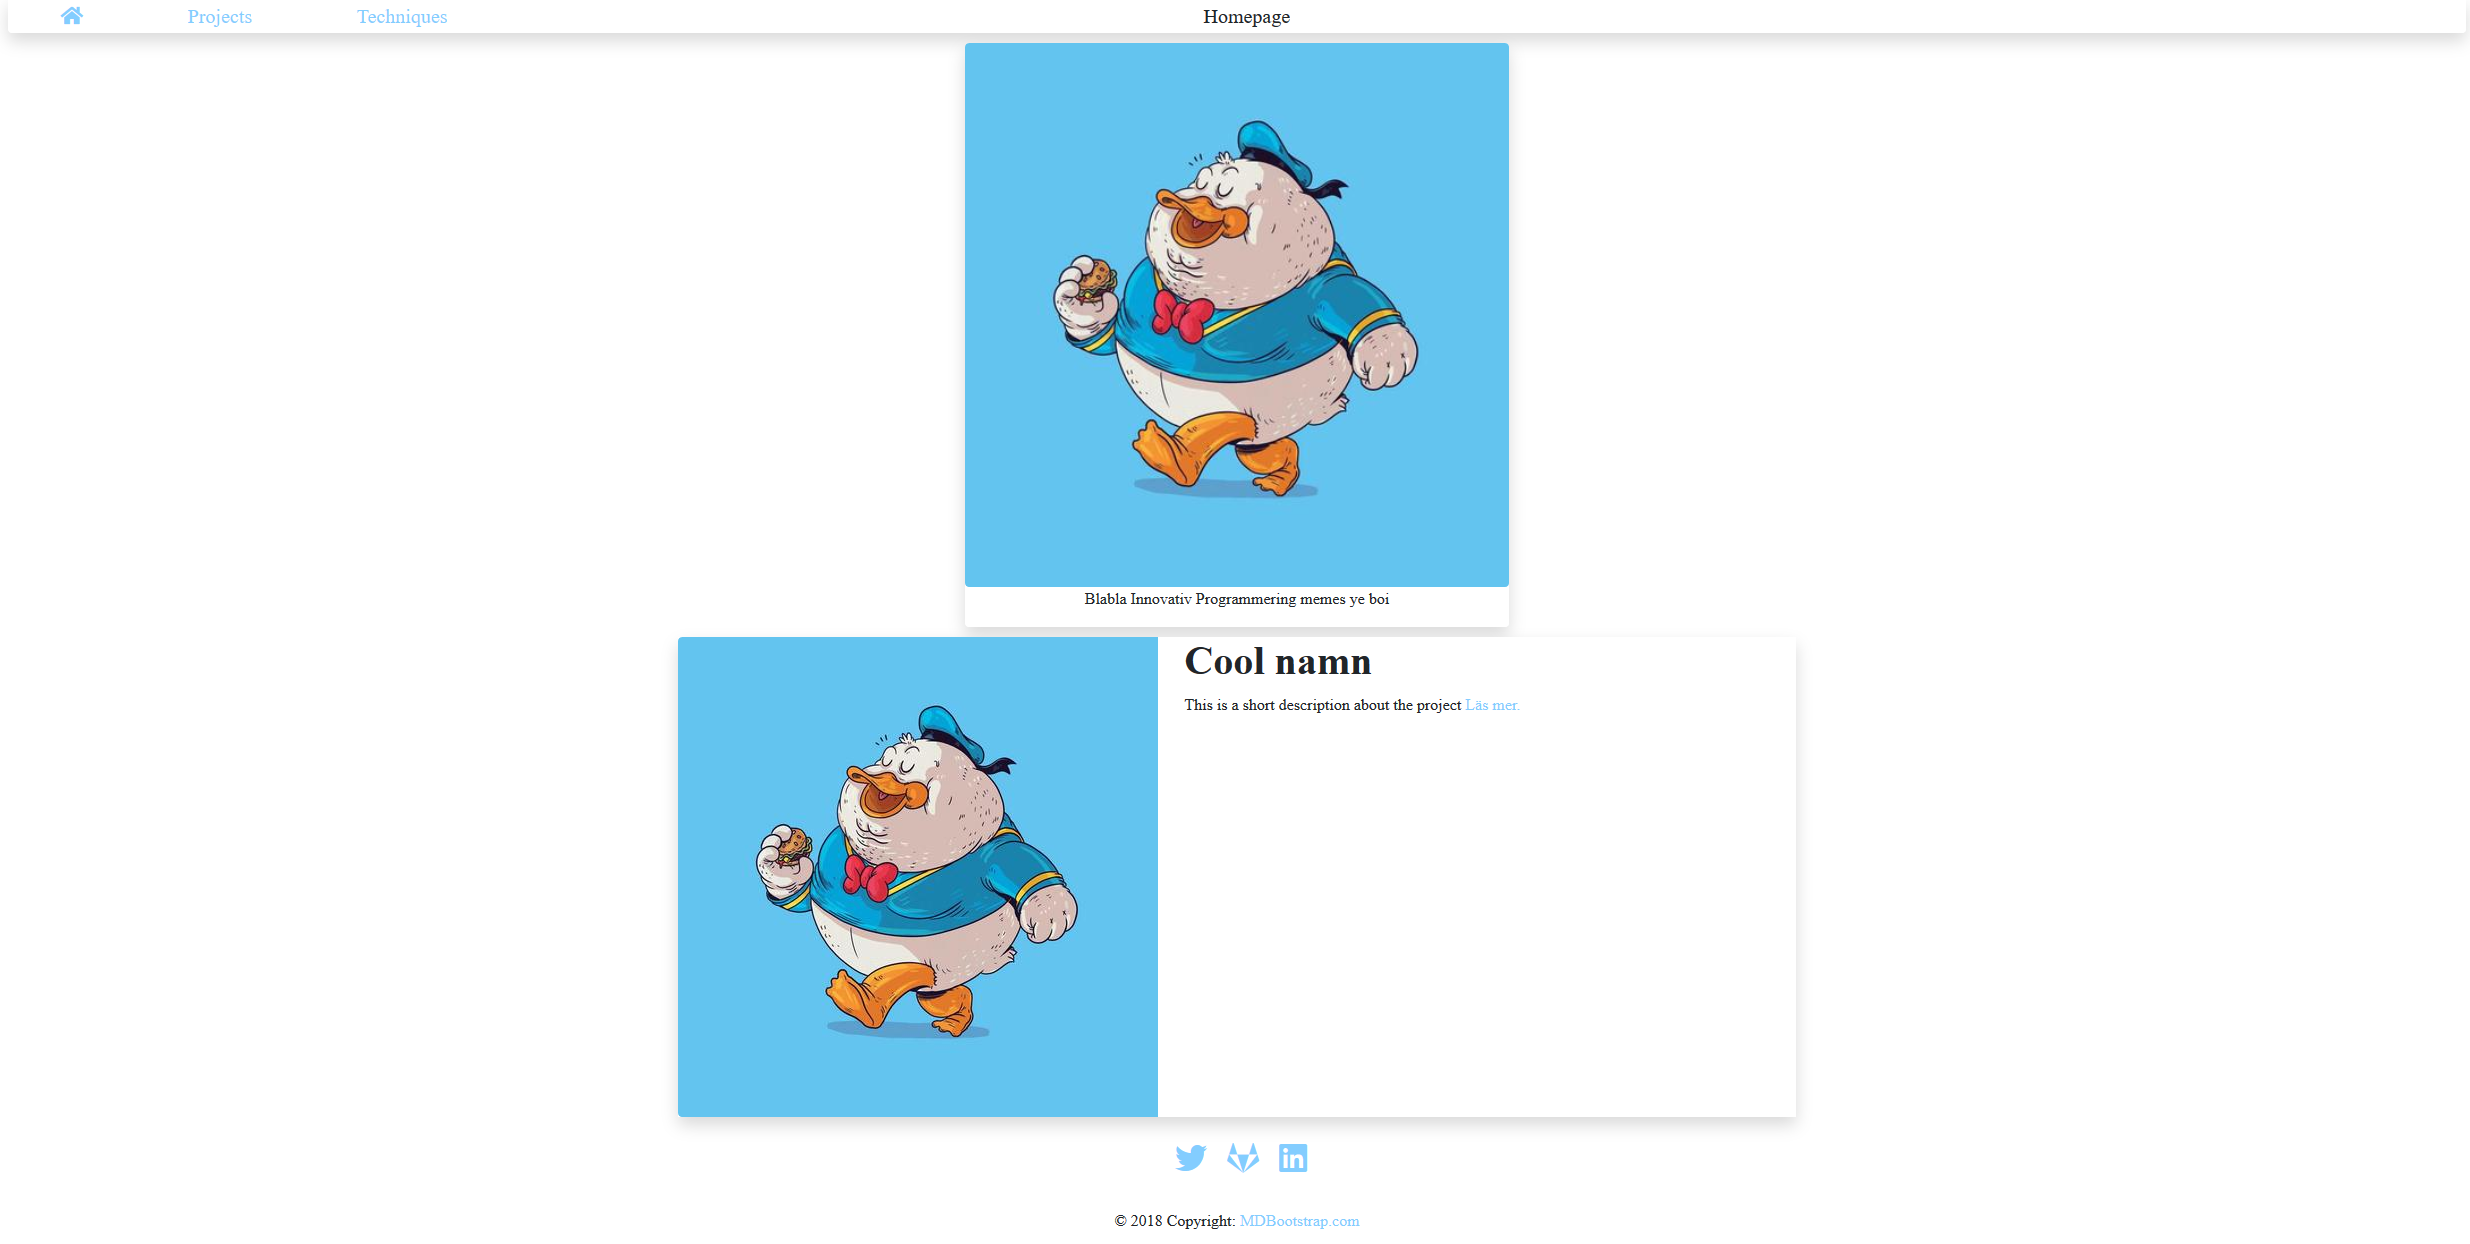
\includegraphics[width=\textwidth, frame]{indexpage.png}
        \caption{Bild på startsidan}
        \label{fig:indexpage}
    \end{subfigure}%
    \hfill
    \begin{subfigure}[b]{0.49\textwidth}
        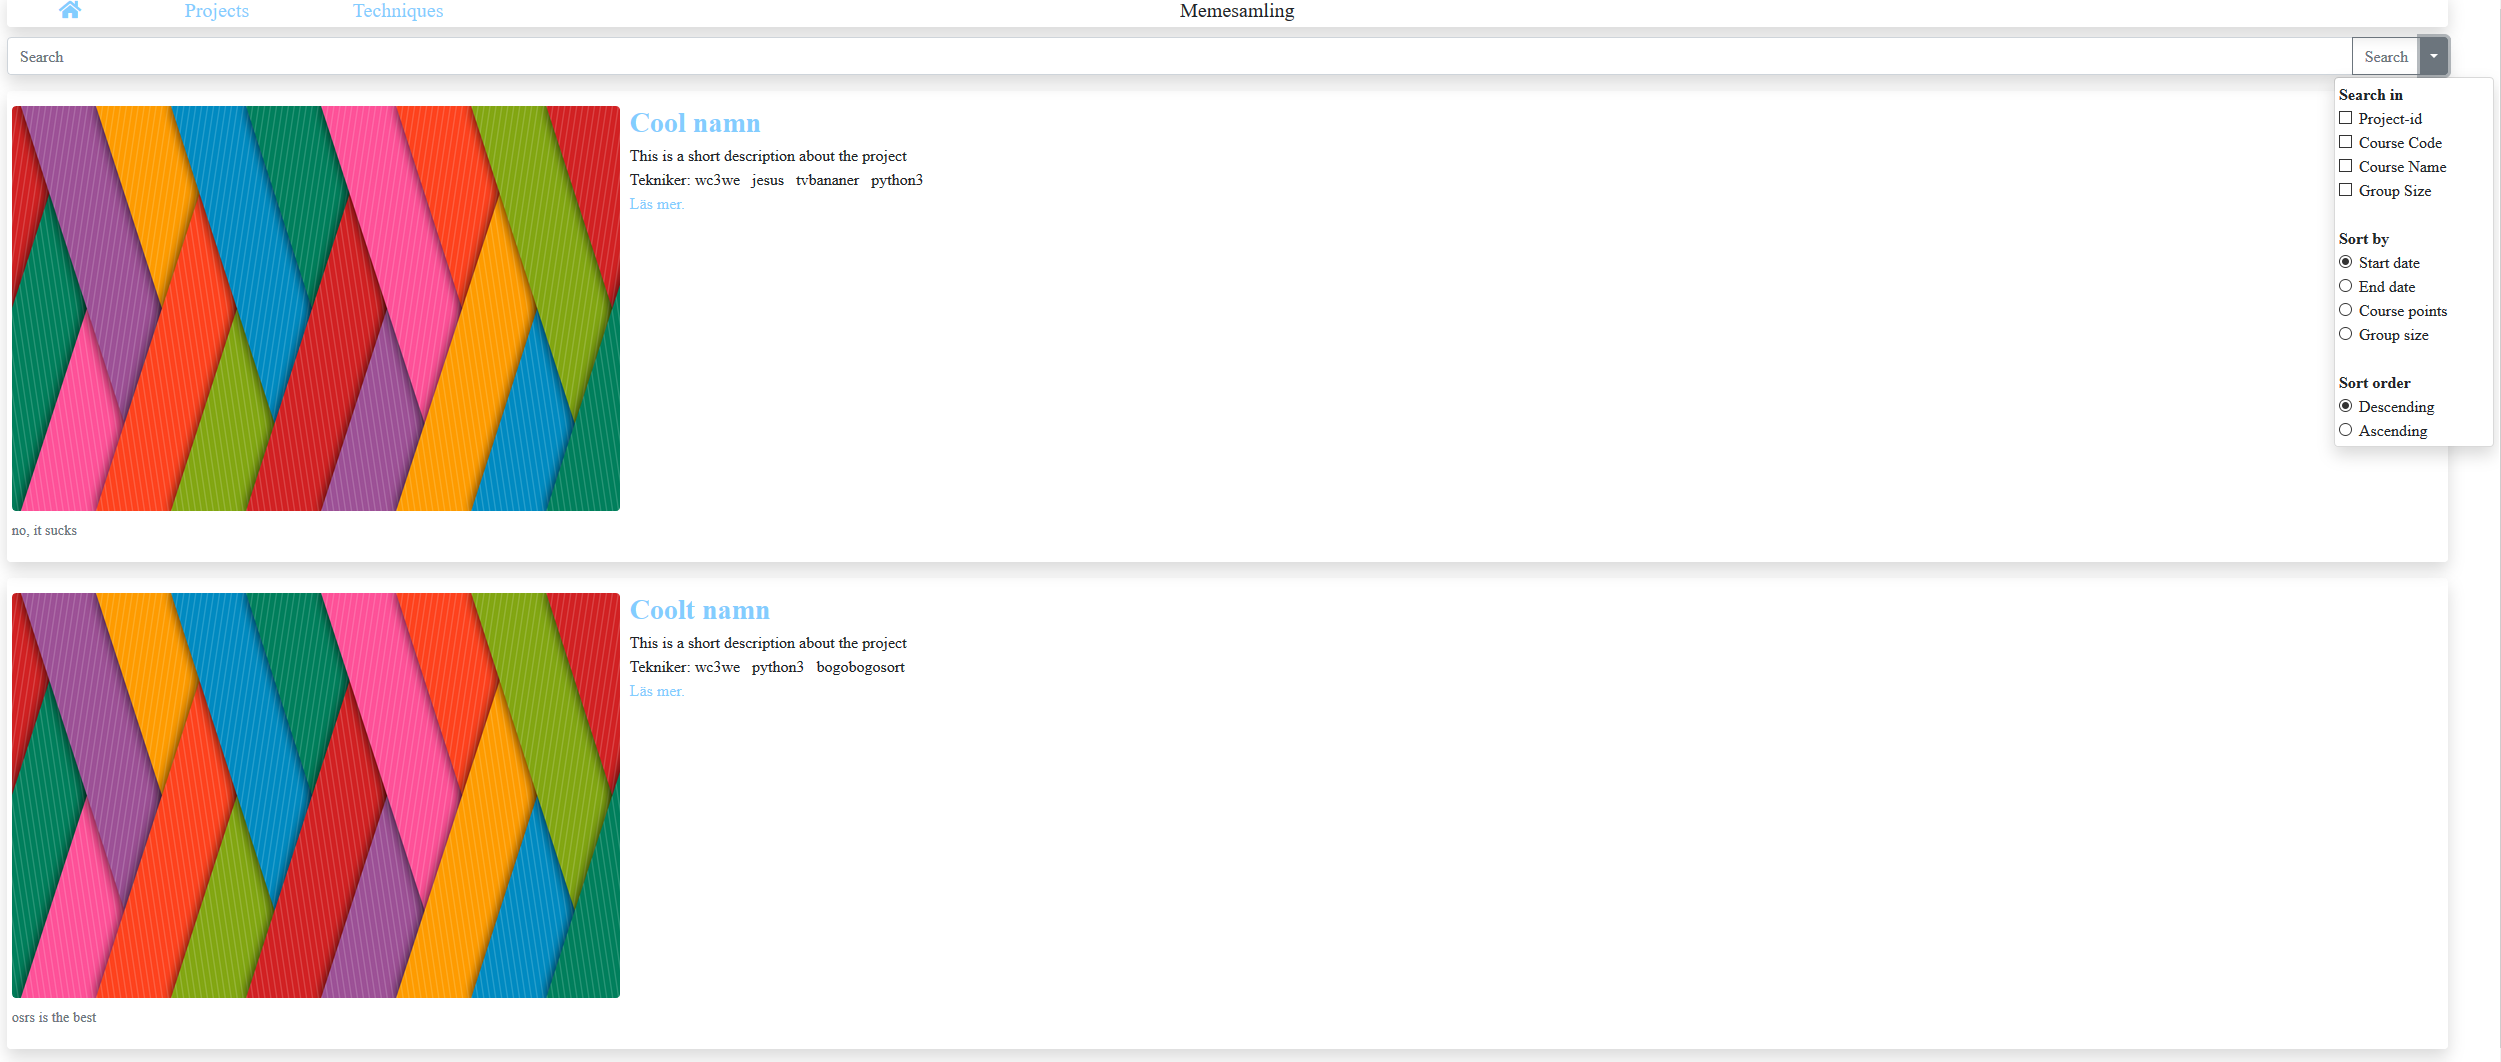
\includegraphics[width=\textwidth, frame]{listpage.png}
        \caption{Bild på söksidan, med \textit{dropdown-meny} nere}
        \label{fig:listpage}
    \end{subfigure}
    \hfill
    \begin{subfigure}[b]{0.49\textwidth}
        
\includegraphics[width=\textwidth, frame]{projectpage.png}
        \caption{Bild på hur en projectsida ser ut}
        \label{fig:projectpage}
    \end{subfigure}
    \hfill
    \begin{subfigure}[b]{0.49\textwidth}
        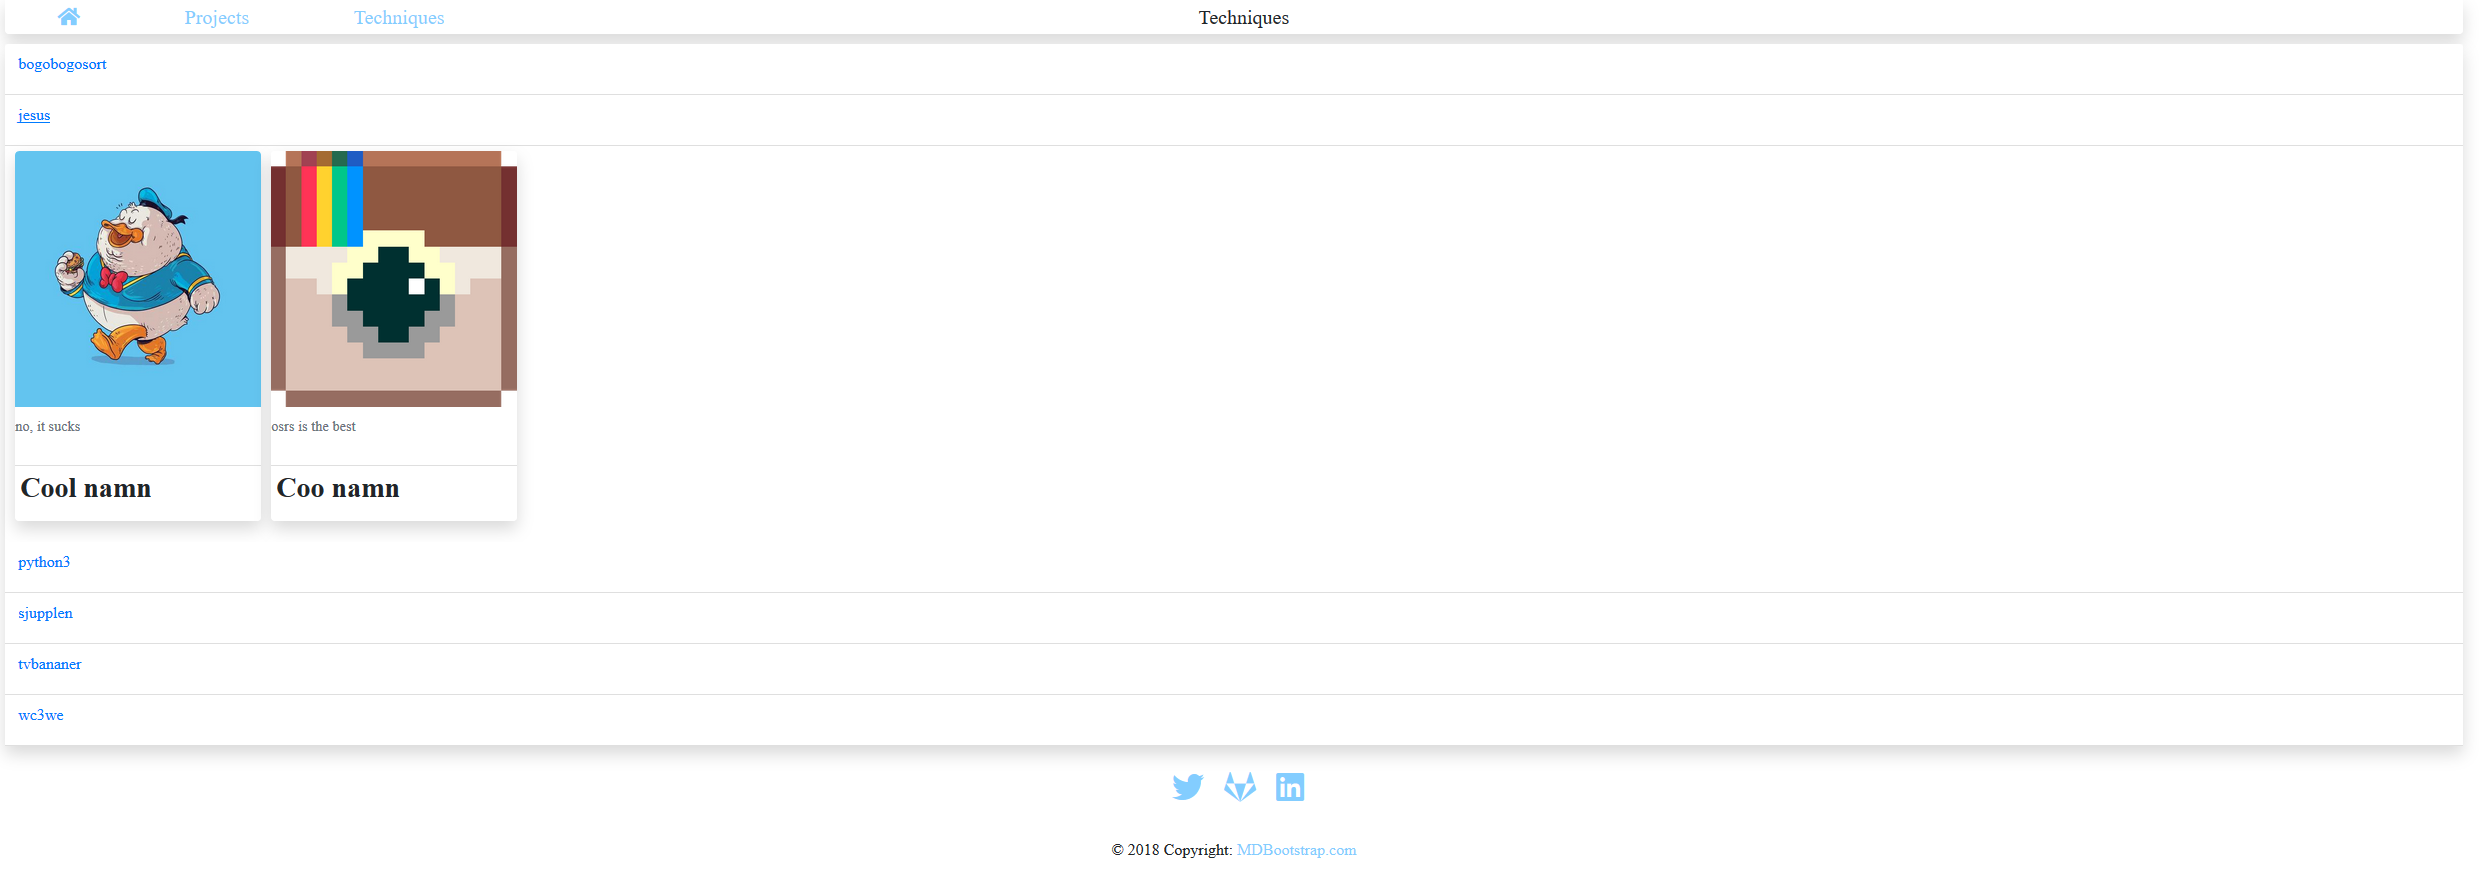
\includegraphics[width=\textwidth, frame]{techniquespage.png}
        \caption{Tekniksidan, med en teknik \enquote{öppen}}
        \label{fig:techniquespage}
    \end{subfigure}
    \hfill
    \begin{subfigure}[b]{0.49\textwidth}
        
\includegraphics[width=\textwidth, frame]{404page.png}
        \caption{404-sidan med relevant information, och en lustig bild}
        \label{fig:404page}
    \end{subfigure}    
    \hfill
    \begin{subfigure}[b]{0.49\textwidth}
        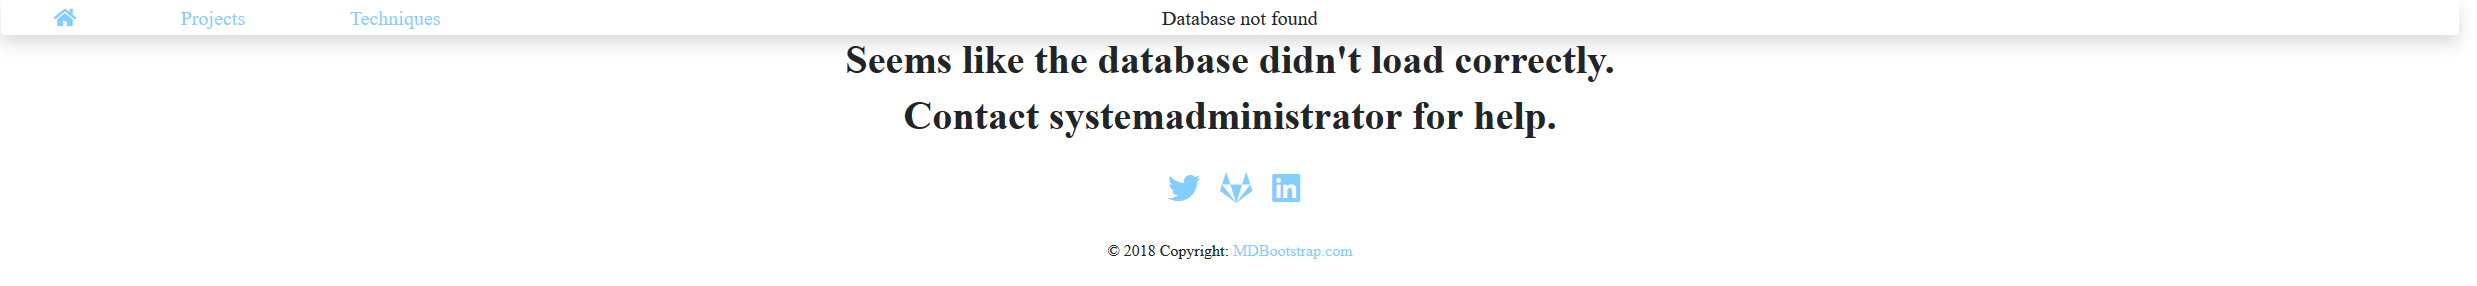
\includegraphics[width=\textwidth, frame]{500page.png}
        \caption{500-sidan med informativ text om vad som hänt.}
        \label{fig:500page}
    \end{subfigure} 
    \label{fig:pagepictures}
\end{figure}
\newpage
\subsection{Index}
\begin{figure}[H]
    \centering
    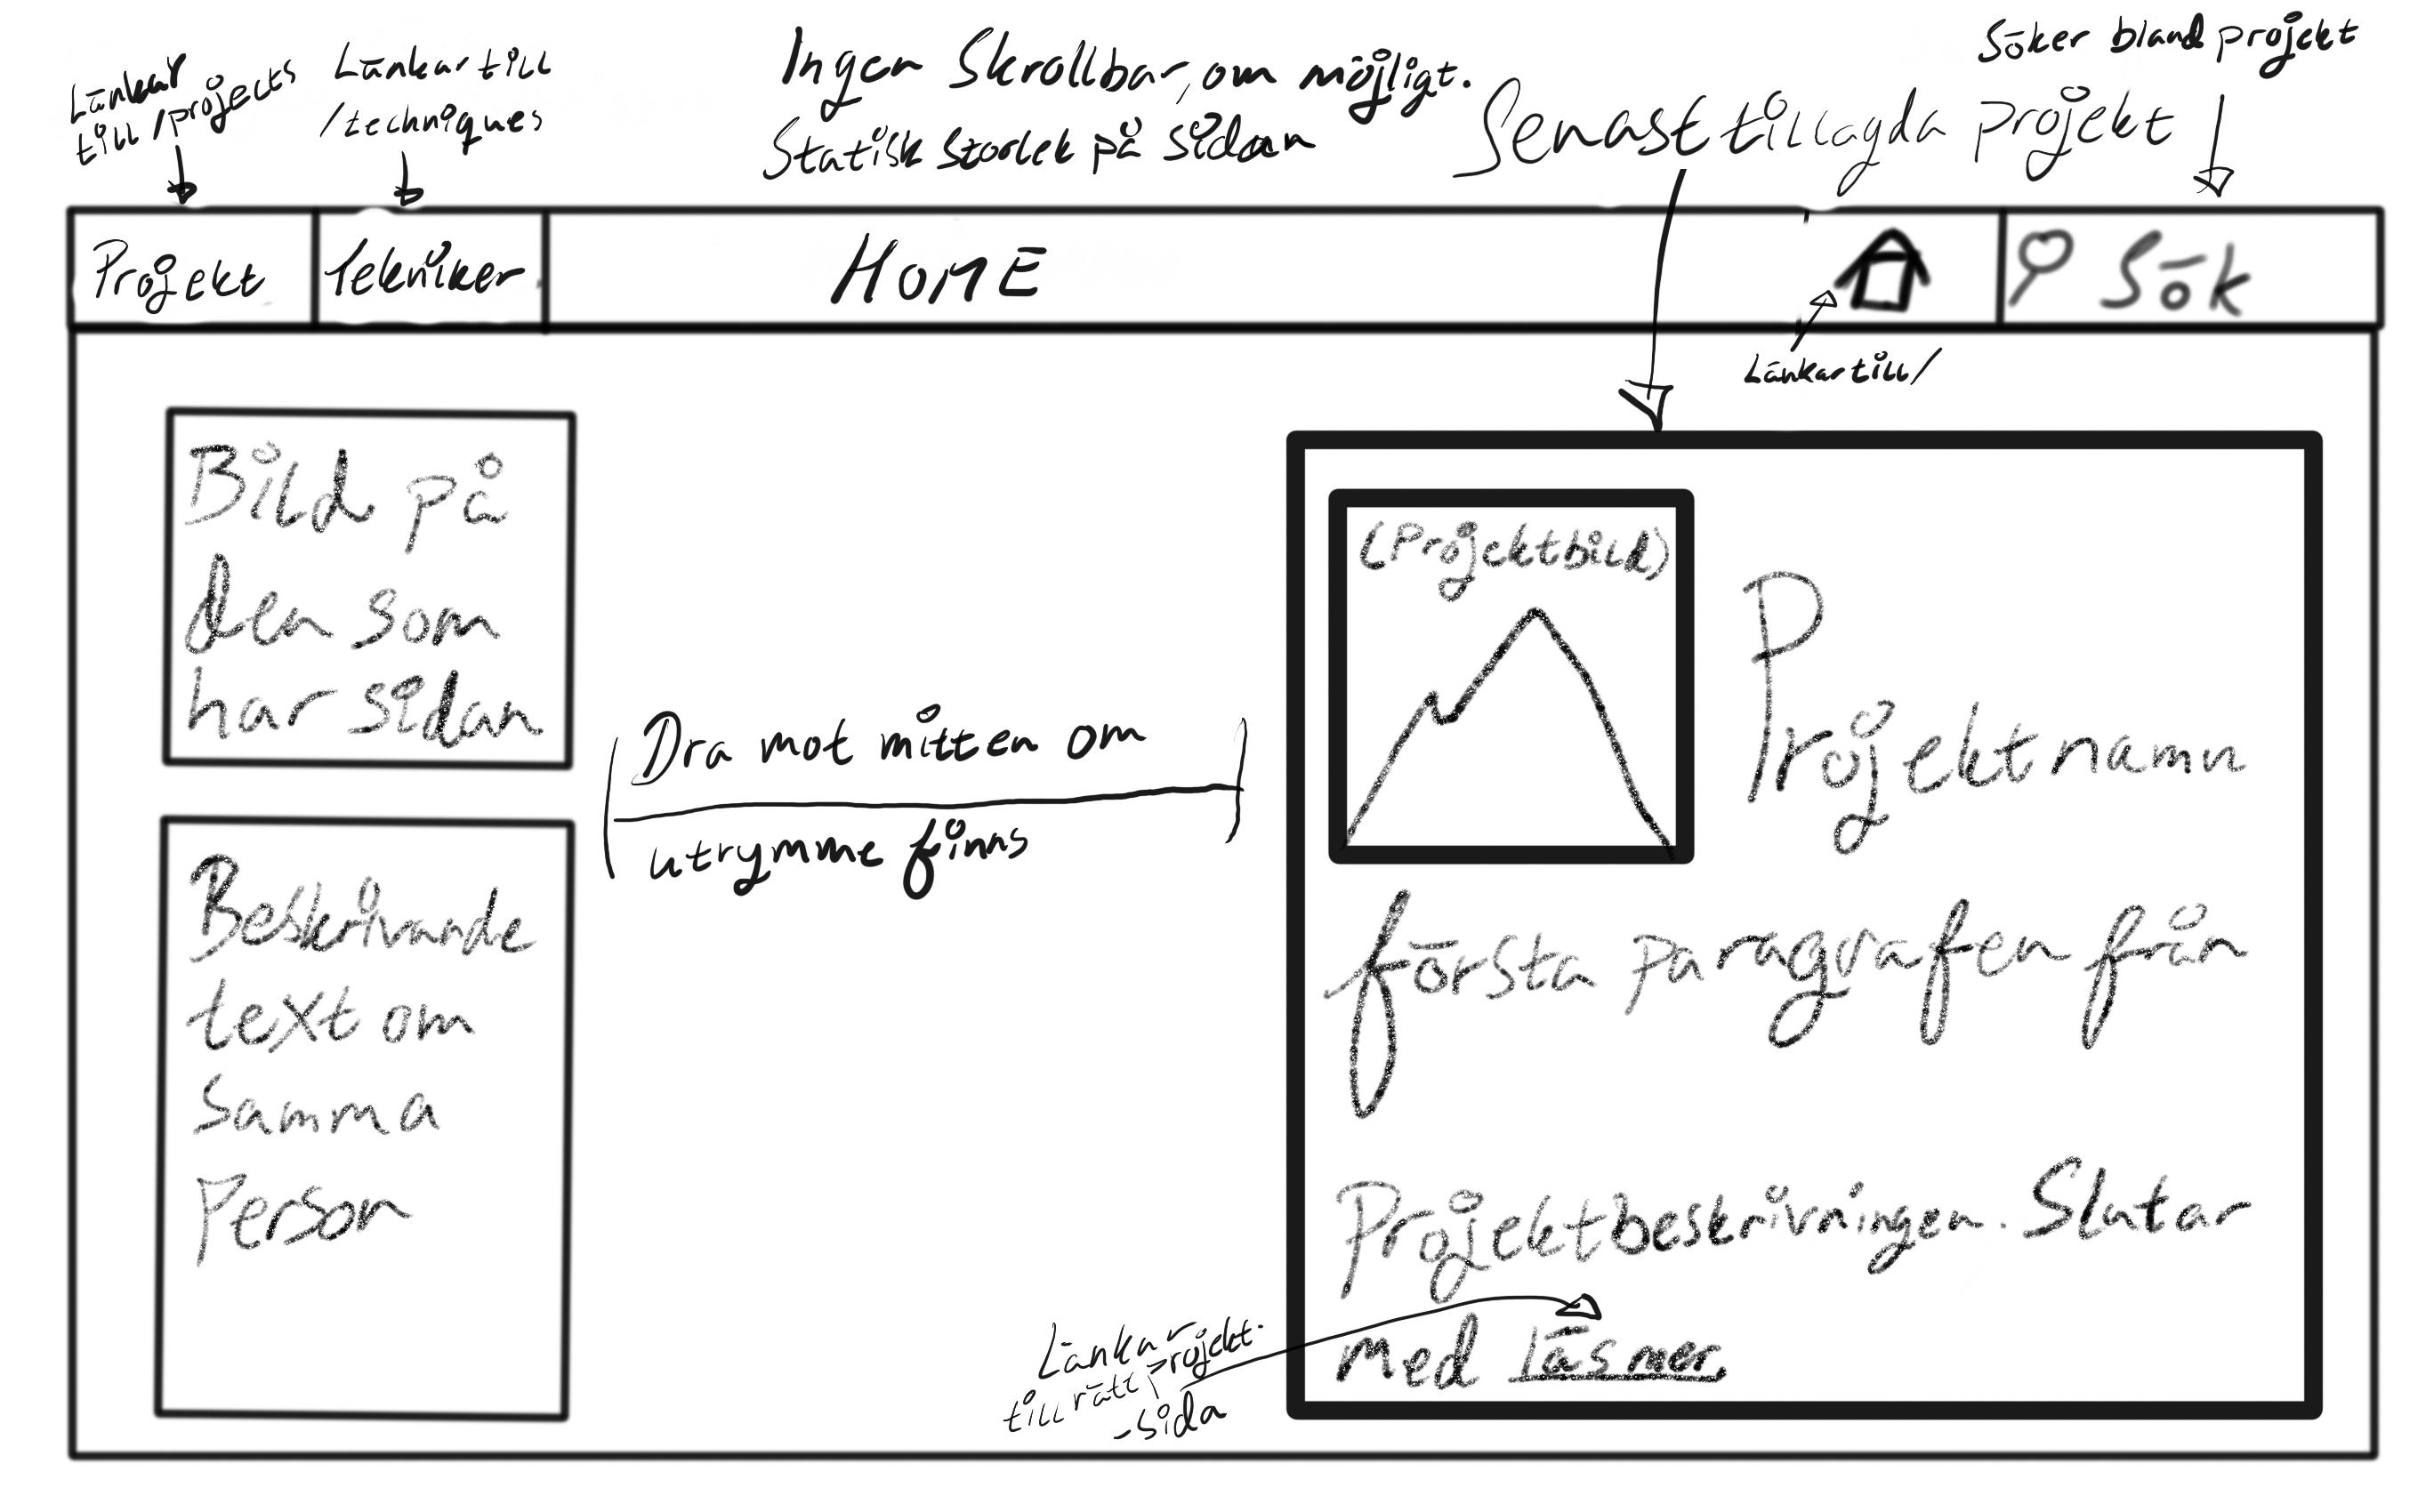
\includegraphics[width=\linewidth]{index.png}
    \caption{Lyckad laddning av start-sidan}
    \label{fig:index}
\end{figure}
Sidan uppfyller alla krav som är listade under kravspecifikation i systemspecifikationen.
Har ej upptäckt några fel under testkörningar eller systemdemonstration.
\subsection{List}
\begin{figure}[H]
    \centering
    
\includegraphics[width=\linewidth]{list.png}
    \caption{Lyckad sökning på project-list-sidan}
    \label{fig:list}
\end{figure}
Alla krav i systemspecifikation har blivit mötta.
Under systemdemonstrationen så stötte vi på problemet att vi inte kunde söka i tekniker.
Det åtgärdade vi genom att ändra i datalagret så att istället för att returnera resultatet av ett
rekursivt anrop på \nameref{sec:checksearch}, se bild \ref{listing:return}, så returnerar vi True om rekursivt anrop på \nameref{sec:checksearch} returnerar True, se bild \ref{listing:if}.
\begin{lstlisting}[caption={retur av rekursivt anrop}, label={listing:return}, language={Python}]
return check_search(sökord, lista)
\end{lstlisting}

\begin{lstlisting}[caption={Retur True om check\_search()}, label={listing:if}, language={Python}]
if check_search(sökord, lista):
    return True
\end{lstlisting}

\subsubsection{Fel i sökning}
\label{sec:nodb}
\begin{figure}[H]
    \centering
    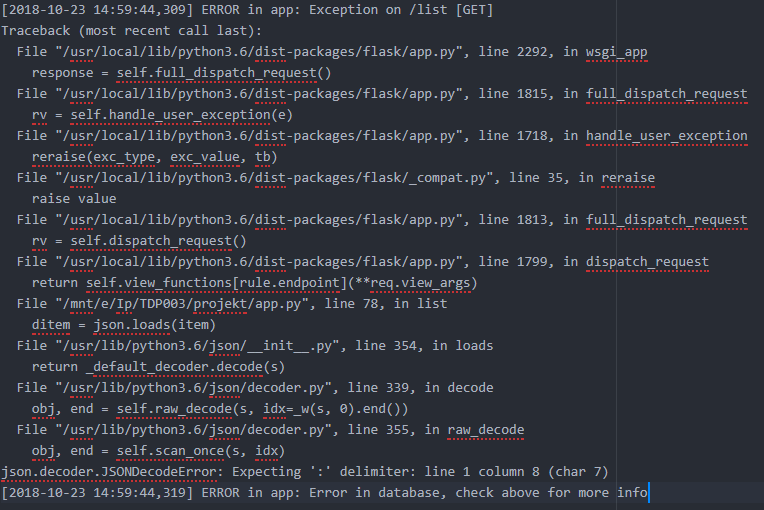
\includegraphics[width=\linewidth]{searchrip.png}
    \caption{Någon har mixtrat i url:en}
    \label{fig:search-error}
\end{figure}
Om man ändrar i url:en i \enquote{http:.../list} så kastas det en 500 server error och man kommer till en sida som tar hand om \textit{500-error}. 
\subsection{Techniques}
\label{sec:techniques}
\begin{figure}[H]
    \centering
    
\includegraphics[width=\linewidth]{ttechniques.png}
    \caption{Lyckad laddning av tekiksidan.}
    \label{fig:techniques}
\end{figure}
Alla krav för tekniksidan har blivit mötta.
Har ej hittat några fel under tester eller systemdemonstration.
\subsection{Project}
\begin{figure}[H]
    \centering
    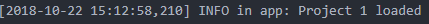
\includegraphics[width=\linewidth]{projekt.png}
    \caption{Lyckad laddning av projektsida.}
    \label{fig:projekt}
\end{figure}
Omdirigering från annan sida kommer leda till lyckad laddning av \enquote{http:.../project/\textit{<id>}}
\subsubsection{Project 404}
\begin{figure}[H]
    \centering
    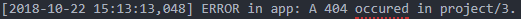
\includegraphics[width=\linewidth]{projekt404.png}
    \caption{Försökte gå in på ett projekt som inte existerar.}
    \label{fig:404projekt}
\end{figure}
Under systemdemonstrationen så märkte vi att det kastades en 500 error om vi försökte komma in på ett projekt som inte existerade genom att ändra i url:en. Det fixade vi genom att lägga till:
\begin{lstlisting}[caption={Kollar om projekt existerar.}, language=Python]
if project == None:
        app.logger.error('A 404 occured in project/{}.'.format(project_id))
        return render_template('page_not_found.html', page_name="Uh oh")
\end{lstlisting}
Detta kollar om projektet vi försöker gå in på existerar i databasen och om det inte gör det så kastar vi en 404 error och laddar 404 sidan, se fig \ref{fig:404projekt}. Detta går att repetera enkelt, genom att i url:en ändra så att det står \enquote{http:.../project/\textit{<id>}} där \textit{<id>} är id på ett projekt som inte finns.
\subsection{Allmän 404}
\begin{figure}[H]
    \centering
    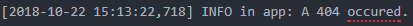
\includegraphics[width=\linewidth]{404.png}
    \caption{Försök att gå in på sida som inte existerar.}
    \label{fig:404}
\end{figure}
Om vi försöker gå in på en sida som inte existerar, till exempel \enquote{http:.../hej}, så kommer vi bli skickade till en 404 sida istället och kasta en error till debug.log, se fig \ref{fig:404}.
\newpage
\section{Log-fil}
\lstinputlisting[firstline=1, lastline=9, language={XML}, label={log:debug.log}, caption={Bit av en log-fil}]{./src_files/debug.log}
I figur \ref{log:debug.log} visar vi en kontrollerad version av hur en \enquote{debug.log} fil. Detta för att visa  vilka log-meddelande vi har skickat in i log-filen, från vårat presentationslager. I ordning uppifrån och ner händer följande:
\begin{itemize}
     \item Nuvarande version av hemsidan skrivs ut.
     \item Index-sidan laddas utan problem.
     \item Sök-sidan laddas utan problem.
     \item Vi söker med \textit{python}, och inga problem upstår under sökning.
     \item \enquote{http:.../project/2} laddas utan problem.
     \item Tekniksidan laddas utan problem.
     \item Försök att ladda \enquote{http:.../project/3}, vilket inte finns, så ett 404-error kastas
     \item Försök att ladda en sida som inte finns, till exempel \enquote{http:.../hej}, som inte finns, så ett 404-error kastas
     \item Sök-sidan laddas utan problem
\end{itemize}
Det som är bra med loggen, är att den beskriver exakt när problemet uppstår, både i datum och klockslag. Detta underlättar ytterligare för att veta vilken version av hemsidan det var som krashade.
\newpage
\section{Datalagret}
För fullständig information om dessa funktioner, se \uline{\href{https://www.ida.liu.se/~TDP003/current/portfolio-api_python3/}{kravspecifikationen}}
\subsection{Load}
\label{sec:load}
\subsubsection{Indata}
Filnamn i \textit{string}-format till en \enquote{.json}-fil som ska laddas in och visas på sidan.
\begin{lstlisting}[caption={Definering av \textbf{load()} funktionen}, language={Python}]
def load(filename):
\end{lstlisting}
\subsubsection{Förväntad utdata}
En \textit{list}-representation av den databas man vill ladda in, enligt hur \textbf{json.load(\textit{fil})} laddar in \textit{.json}-filer. 
\subsubsection{Möjliga fel}
Om filen inte finns, returnerar \textbf{load} \textit{None}, vilket resulterar i att sidan kraschar och man skickas till en \textit{500}-error sida, så att man får lite information om felet.
\begin{lstlisting}[caption={Hantering när den inte hittar filen}, language={Python}]
 except FileNotFoundError:
        return None
\end{lstlisting}

\subsection{Get project count}
\subsubsection{Indata}
Databasen som vi laddar med \uline{\nameref{sec:load}} representerad av en \textit{list}.
\begin{lstlisting}[caption={Definering av \textbf{get\_project\_count()} funktionen.}, language=Python]
def get_project_count(db):
\end{lstlisting}
\subsubsection{Förväntad utdata}
Antalet projekt i databasen. 
\subsubsection{Möjliga fel}
Vi har inte hittat något som kan gå fel i denna funktion.

\subsection{Get project}
\subsubsection{Indata}
Skicka in en databas, efter att den laddats med hjälp av \uline{\nameref{sec:load}}, och ett projekt-id på formen \textit{integer}.
\begin{lstlisting}[caption={Definering av \textbf{get\_project()} funktionen.}, language=Python]
def get_project(db, id):
\end{lstlisting}
\subsubsection{Förväntad utdata}
Ett projekt så som det representeras i databasen, i vårat fall är det en \textit{dictionary} med data i.
\subsubsection{Möjliga fel}
Om project-id inte finns i database, skickas en \textit{None-type}.  
\begin{lstlisting}[caption={Retur ifall inget projekt hittas}, language={Python}]
return None
\end{lstlisting}
\subsection{Get latest project}
\subsubsection{Indata}
Skickar in databasen som laddas med \uline{\nameref{sec:load}}.
Projekten sorteras efter datum med hjälp av \uline{\nameref{sec:search}} för att få det senast skapade projektet.
\begin{lstlisting}[caption={Definering av \textbf{get\_latest\_project()} funktionen.}, language=Python]
def get_latest_project(db):
\end{lstlisting}
\subsubsection{Förväntad utdata}
Det senaste projektet ur databasen på samma format som det existerar i databasen.
\subsubsection{Möjliga fel}
Om datumformatet på projektet inte stämmer överens med det formatet som vi använder så kommer inte
projektet att sorteras på rätt sätt. Då kommer de att komma i fel ordning.

\subsection{Search}
\label{sec:search}
Använder sig av två underfunktioner \uline{\nameref{sec:searchproject}} och \uline{\nameref{sec:checksearch}}.
\subsubsection{Indata}
\textbf{search()} tar in mycket data, så de listas nedan, med en kort beskrivning.
\begin{itemize}
    \item db -> Databas, som fås från \uline{\nameref{sec:load}}.
    \item sort\_by -> En \textit{string} som bestämmer vilket datafält man sorterar på.
    \item sort\_order -> En \textit{string} som bestämmer om man sorterar efter \enquote{stigande} eller \enquote{fallande}.
    \item techniques -> En \textit{lista} med tekniker som man vill söka efter i projekten.
    \item search -> Fritext på \textit{string}-format.
    \item searchfield -> En \textit{lista} med \textit{string}, som bestämmer i vilka datafält man söker med \enquote{search}
\end{itemize}
\begin{lstlisting}[caption={Definering av \textbf{search()} funktionen.}, language=Python]
def search(db, sort_by='start_date', sort_order='desc',
           techniques=None, search=None, searchfield=None):
\end{lstlisting}
\subsubsection{Förväntad utdata}
Databasen filtrerad på de sökkriterier som skickats med, sorterad i antingen \enquote{stigande} eller \enquote{fallande}.
\subsubsection{Möjliga fel}
Om \uline{\nameref{sec:load}} returnerar \textit{None} kommer \uline{\nameref{sec:search}} att krascha. Kolla på \uline{\nameref{sec:nodb}} i \uline{\nameref{sec:presentation}} för mer info om vad som händer då.

\subsection{Search project}
\label{sec:searchproject}
\subsubsection{Indata}
Tar in ett projekt representerat av en \textit{dictionary}, ett sökord representerat av en \textit{string} och ett sökfälts-filter representerat av en \textit{string}, om man användaren vill filtrera på det. \begin{lstlisting}[caption={Definering av search\_project()}, language={Python}]
def search_project(project, search_word, searchfield):
\end{lstlisting}
\subsubsection{Förväntad utdata}
Om sökordet finns i projektet, returnerar den \textit{True}, annars \textit{False}.
\subsubsection{Möjliga fel}
Då denna funktion fungerar som en mellanhand mellan \uline{\nameref{sec:search}} och \uline{\nameref{sec:checksearch}}, kastas det inga fel i denna funktion.
\subsection{Check search}
\label{sec:checksearch}
\subsubsection{Indata}
Tar in ett sökord, representerat av en \textit{string}, och ett datafält, representerat av en \textit{list}, en \textit{integer}, eller en \textit{string}, för att söka i. 
\begin{lstlisting}[caption={Definering av \textbf{check\_search()} funktionen.}, language=Python]
def check_search(search_word, item):
\end{lstlisting}
\subsubsection{Förväntad utdata}
Antingen så returnerar vi \textit{True} eller \textit{False} beroende på om sökordet matchar datafältet eller inte.
\subsubsection{Möjliga fel}
Om vi skulle få in en \textit{dictionary} som datafält så kommer det krascha då vi inte hanterar detta fall. 

\subsection{Get techniques}
\label{sec:gettechniques}
\subsubsection{Indata}
Skickar in databasen som laddas med \uline{\nameref{sec:load}} för att sedan ta ut alla unika tekniker som används i projekten.
\begin{lstlisting}[caption={Definering av get\_techniques()}, language={Python}]
def get_techniques(db):
\end{lstlisting}
\subsubsection{Förväntad utdata}
En sorterad lista med alla unika tekniker som använts i projekten i databasen.
\subsubsection{Möjliga fel}
Vi har ej hittat några möjliga fel under testerna av denna funktion. Blir något fel så händer det innan denna funktion kan anropas.

\subsection{Get technique stats}
\subsubsection{Indata}
Skickar in databasen och alla tekniker vi får ut från \uline{\nameref{sec:gettechniques}} för att sedan sortera vilka tekniker som används för vilka projekt.
\begin{lstlisting}[caption={Definering av get\_technique\_stats()}, language={Python}]
def get_technique_stats(db):
\end{lstlisting}
\subsubsection{Förväntad utdata}
En dictionary med tekniker som nyckel med projekten som använder tekniken som item till nyckeln i en lista. 
\subsubsection{Möjliga fel}
Vi lägger endast till tekniker som redan blivit filtrerade i \uline{\nameref{sec:gettechniques}} så här har vi inte hittat några möjliga fel.
\subsubsection{Avvikelse från specifikation}
\textbf{get\_technique\_stats()} avviker från  specifikationen i det faktum att vi i listan för varje teknik lägger till hela projektet, istället för bara projektnamn och projektid. Detta har vi ändrat för att förenkla för oss på \uline{\nameref{sec:techniques}}, så att vi inte behöver skicka med för många variabler. Vår kod ser ut som i figur \ref{lsst:gt1}, medan koden i figur \ref{lsst:gt2} är enligt kravspecifikation.
\begin{lstlisting}[caption={Vår lösning på get\_technique\_stats().}, label={lsst:gt1}, language=Python]
if technique in item["techniques used"]
    technique_stats[technique].append(item)
\end{lstlisting}
\begin{lstlisting}[caption={Lösningen enligt kravspecifikationen.}, label={lsst:gt2}, language=Python]
if technique in item["techniques_used"]:
    technique_stats[technique].append({"id":item["project_id"], "name":item["project_name"]})
\end{lstlisting}
\end{document}
